\documentclass[11pt,a4paper,twocolumn]{article}

% === Core Packages ===
\usepackage[margin=2cm]{geometry}
\usepackage[utf8]{inputenc}
\usepackage[T1]{fontenc}
\usepackage{times}
\usepackage{amsmath,amssymb}
\usepackage{graphicx}
\usepackage{booktabs}
\usepackage{float}
\usepackage{enumitem}
\usepackage{tikz}
\usepackage{pgfplots}
\pgfplotsset{compat=1.18}
\usetikzlibrary{arrows.meta,shapes.geometric,positioning,calc,decorations.markings,fit,backgrounds}

% === Citation (IEEE style) ===
\usepackage[numbers,sort&compress]{natbib}
\bibliographystyle{IEEEtranN}

% === Hyperref ===
\usepackage[hidelinks]{hyperref}
\usepackage{xurl}

% === Settings ===
\setlength{\parindent}{1em}
\setlength{\parskip}{0.3em}

% === Title ===
\title{\textbf{Hajautettu mainejärjestelmä:\\Viitekehys yhteiskunnan luonnolliselle järjestäytymiselle}}
\author{Pavel Kudrna\\Praha, Tšekki\\Luonnos v1 --- maaliskuu 2026}
\date{}

\begin{document}
\maketitle

% ============================================================
% ABSTRACT
% ============================================================
\begin{abstract}
Oikeudentunto---vakaumus siitä, että vääryydet oikaistaan ja ansiot palkitaan---on yhteiskunnan vahvin koossapitävä voima. Kun keskitetyt hallintoinstituutiot eivät kykene tuottamaan tätä tunnetta, koska oikeuden toteuttamisen kustannus ylittää itse oikeuden arvon, sosiaalinen koheesio rapautuu. Nykyiset institutionaaliset rakenteet epäonnistuvat merkittävän riitaluokan ratkaisemisessa järjestelmällisesti samalla tavalla kuin keskusjohtoinen suunnittelu epäonnistuu resurssien kohdentamisessa: informaation epäsymmetrian, puuttuvien takaisinkytkentöjen ja päätöksentekijöiden ja heidän päätöstensä seurausten välisen katkoksen kautta. Tämä artikkeli esittelee maineeseen perustuvan sosiaalisen verkoston (Reputation Social Network, RSN): hajautetun, korruptoitumattoman ja sensuuria kestävän viestintäkerroksen, joka rakentuu hajautetuille tunnisteille (Decentralized Identifiers, DID) ja mahdollistaa salanimellä toimiville osallistujille todellisesta käyttäytymisestä kertovan mainetiedon julkaisemisen, todentamisen ja kuluttamisen. Ydinmekanismi nojaa kolmeen suunnitteluperiaatteeseen: (1)~epäsymmetriseen kustannusrakenteeseen, jossa mainetiedon lukeminen on halpaa mutta kirjoittaminen edellyttää todennettavaa ponnistelua; (2)~epädeterministiseen todentajan valintaprotokollaan, joka perustuu johdonmukaiseen tiivistämiseen ja hinnoittelee radikaalit väitteet kasvavien iteraatiokustannusten kautta; ja (3)~markkinavetoiseen maineauktoriteettimalliin, jossa yksityiset todentajat panttaavat kertyneen maineensa hyväksymiensä väitteiden paikkansapitävyyden puolesta. Näin syntyvä arkkitehtuuri tuottaa emergentin meritokratian ilman keskitettyä koordinointia ja mahdollistaa asteittaisen, peruutettavissa olevan siirtymäpolun nykyisistä valtion hallinnoimista järjestelmistä.
\end{abstract}

% ============================================================
% 1. INTRODUCTION
% ============================================================
\section{Johdanto}

\subsection{Keskitetyn luottamuksen ongelma}

Nykyaikainen hallinto nojaa perustavaan oletukseen: että keskitetyt instituutiot voivat välittää luottamusta tuntemattomien välillä laajassa mittakaavassa. Tuomioistuimet ratkaisevat riitoja. Rekisterit vahvistavat omistusoikeuden. Sääntelyelimet valvovat standardeja. Nämä instituutiot suunniteltiin aikakautena, jolloin informaatio oli niukkaa, viestintä hidasta ja auktoriteetin delegointi keskuselimelle oli ainoa toteuttamiskelpoinen koordinointimekanismi. Keskitetty hallinto kuitenkin epäonnistuu samoista rakenteellisista syistä kuin keskusjohtoinen suunnittelu: informaation epäsymmetria, puuttuvat takaisinkytkennät sekä päätöksentekijöiden ja heidän päätöstensä seurausten välinen katkos.

Oletus pettää esimerkiksi silloin, kun institutionaalisen välityksen kustannus ylittää riidan arvon. Ajatellaan vuokralaista, joka havaitsee, että hänen vuokra-asunnostaan puuttuu lain edellyttämä sähköturvallisuustodistus---puute, joka aiheuttaa välittömän hengenvaaran. Vuokralaisen laillinen oikeus purkaa sopimus on kiistaton. Silti tuon oikeuden toteuttamisen kustannus tuomioistuinjärjestelmän kautta ylittää vakuuden ja maksettavien vahingonkorvausten rahallisen arvon, vaikka mukaan laskettaisiin mahdollinen lakisääteinen korvaus~\cite{czcourtfees}. Rationaalinen vastaus on kärsiä tappio ja vetäytyä.

Tämä ei ole patologinen ääritapaus. Se on oletusarvoinen kokemus merkittävässä riitaluokassa, jossa vahinko on todellinen mutta rahallinen panos jää sen kynnyksen alle, jonka yläpuolella institutionaalinen täytäntöönpano tulee taloudellisesti järkeväksi. Tuloksena on järjestelmä, joka rakenteellisesti suosii pahantekijöitä: ne, jotka vahingoittavat muita tämän kynnyksen alittavissa määrin, voivat toimia rankaisematta, koska oikeuden hakemisen kustannus lankeaa vahinkoa kärsineelle osapuolelle.

Yllä oleva esimerkki on peräisin kirjoittajan oikeudellisesta ympäristöstä---Tšekin siviilioikeusjärjestelmästä. Muissa oikeusperinteissä---ennakkopäätöksiin nojaava common law, tapaoikeus, sekajärjestelmät---oikeus epäonnistuu eri tavoin ja eri asteissa riippuen lainkäyttöalueen kulttuurisista ja menettelyllisistä erityispiirteistä. Lukijat tunnistanevat vastaavia esimerkkejä omasta kontekstistaan. Rakenteellisesti universaalia on kuvio: riidat, joiden arvo jää taloudellisesti järkevän täytäntöönpanon kynnyksen alle, päättyvät siihen, että vahinkoa kärsinyt osapuoli kantaa tappion. RSN ei lupaa täydellistä oikeutta---se vain vähentää sitä rakenteellista etua, jonka pahantekijät saavat, kun institutionaalinen täytäntöönpano on epätaloudellista.

\subsection{Miksi olemassa olevat ratkaisut jäävät vajaiksi}

\textbf{Hajautetun identiteetin (DID) viitekehykset}~\cite{did2022} tarjoavat kryptografisia mekanismeja itsemääräisen identiteetin hallintaan, mutta keskittyvät ensisijaisesti identiteetin todentamiseen käsittelemättä laajempaa kysymystä käyttäytymiseen perustuvasta maineesta.

\textbf{Sielusidonnaiset tunnukset (Soulbound Tokens, SBT)}~\cite{weyl2022} tavoittavat oivalluksen siitä, että maine on siirtokelvotonta, mutta nojaavat lohkoketjuinfrastruktuuriin, jolla on skaalautuvuusrajoitteita, eivätkä käsittele tiedon syöttämistä ohjaavia taloudellisia kannustimia. Vastaavat käsitteet, kuten ansiotunnukset (esim. Liberland), jakavat samankaltaisen filosofian mutta pysyvät sidottuina tiettyihin lainkäyttöalueen viitekehyksiin.

\textbf{Hajautetut autonomiset organisaatiot (Decentralized Autonomous Organizations, DAO)}~\cite{buterin2014} toteuttavat hallinnon älysopimusten kautta, mutta toistavat plutokraattista dynamiikkaa, jossa vaikutusvalta on suhteessa pääomaan. Neliöllinen äänestäminen~\cite{buterin2019} lieventää tätä osittain mutta rajoittaa käytännön omaksumista. DAO:t kohtaavat myös perustavan \emph{oraakkeliongelman}: älysopimukset eivät voi luotettavasti todentaa todellisen maailman tiloja ilman luotettua ulkoista lähdettä, eikä tähän ongelmaan ole yleistä ratkaisua lohkoketjuarkkitehtuurin sisällä.

Mikään olemassa oleva järjestelmä ei yhdistä hajautusta, sensuurin kestävyyttä, salanimisyyttä, todennettavaa syöttämisen kustannusta ja emergenttiä konsensusta.

\subsection{Tutkimuksen kontribuutiot}

Tämä artikkeli tekee seuraavat kontribuutiot:
\begin{enumerate}[nosep]
\item \textbf{Maineeseen perustuvan sosiaalisen verkoston (RSN)} määrittely: hajautettu protokolla, joka laajentaa DID-viitekehystä tukemaan kaksisuuntaista mainevaihtoa.
\item \textbf{Epädeterministinen todentajan valintaprotokolla}, joka perustuu johdonmukaiseen tiivistämiseen~\cite{karger1997}.
\item \textbf{Kalliin radikalismin periaate}, joka hinnoittelee väitteet niiden etäisyyden mukaan verkoston konsensuksesta kolmen kasautuvan kustannuskanavan kautta.
\item \textbf{Maineauktoriteettimalli}, jossa on epäsymmetriset kannustimet ja jossa väärä hyväksyntä maksaa katastrofaalisesti enemmän kuin legitiimit maksut.
\item \textbf{Asteittainen siirtymäpolku} rinnakkaisen finanssi-infrastruktuurin kautta.
\end{enumerate}

% ============================================================
% 2. DESIGN PRINCIPLES
% ============================================================
\section{Suunnitteluperiaatteet}

RSN-arkkitehtuuria rajaa viisi neuvottelematonta suunnitteluperiaatetta.

\textbf{Jatkuvuus ja kehitys.} Järjestelmä toimii rinnakkain olemassa olevien instituutioiden kanssa määrittelemättömän pituisen siirtymäkauden ajan. Siirtymän on oltava peruutettavissa jokaisessa vaiheessa.

\textbf{Vapaaehtoisuus ja vastuu.} Osallistuminen on vapaaehtoista, mutta vapaaehtoisuuteen kytkeytyy vastuu: osallistuja, joka ottaa haltuunsa institutionaalisen tehtävän, ottaa samalla kannettavakseen siihen liittyvät velvoitteet.

\textbf{Moninaisuus ja kulttuurinen neutraalius.} Konsensus syntyy kaksisuuntaisista vuorovaikutuksista, ei järjestelmän suunnittelijoiden asettamista ennalta määrätyistä säännöistä.

\textbf{Kestävyys ja sensuurin vastustuskyky.} Verkoston sensuroinnin kustannuksen on ylitettävä sen sietämisen kustannus. Vain täysi totalitarismi---turmiollisin poliittisin ja taloudellisin kustannuksin---voi tukahduttaa järjestelmän.

\textbf{Konsensus ja täytäntöönpano.} Järjestelmä sisällyttää inhimilliset taipumukset pikkumaisuuteen, ilkeyteen ja kostonhaluiseen tyydytykseen kantaviksi ominaisuuksiksi. Väärinkäytöstä ei kielletä; se hinnoitellaan.

% ============================================================
% 3. SYSTEM OVERVIEW
% ============================================================
\section{Järjestelmän yleiskuvaus}

\subsection{Maineeseen perustuva sosiaalinen verkosto}

RSN on hajautettu, vertaisverkkoon (peer-to-peer) perustuva viestintäkerros, jossa osallistujat vaihtavat todennettavaa tietoa todellisesta käyttäytymisestä. Sen määrittelevät ominaisuudet ovat: hajautettu ja sensuroimaton infrastruktuuri; salanimellä osallistuminen DID:ien kautta; epäsymmetrinen kustannusrakenne (lukeminen halpaa, kirjoittaminen kallista); kryptografinen todennettavuus; ja \textbf{standardituki}---koneluettavat muodot verkostossa leviävälle tiedolle, auktoriteettien tarjoamille palveluille (väitteen kokoaminen, hyväksyntä, todistajapalvelu) sekä käytäntömuodolle, joka sisältää säännöt vastapuolen maineen arvioimiseen ja käytäntöristiriidan (ilmoitetun ja todellisen käyttäytymisen välillä) riskin arviointiin.

\subsection{Arkkitehtuurin komponentit}

RSN koostuu neljästä pääkomponentista (kuva~\ref{fig:architecture}):
\begin{enumerate}[nosep]
\item \textbf{DID-kerros.} Osallistujien identiteetit ilmoitettuine sääntöineen, mainemetadatoineen ja verkostoreitityksineen.
\item \textbf{Väiteprotokolla.} Jäsennelty muoto todellisen maailman tapahtumia koskevien väitteiden julkaisemiseen.
\item \textbf{Todennusverkosto.} Hajautettu protokolla todentajien osoittamiseen johdonmukaisen tiivistämisen avulla.
\item \textbf{Maineen aggregointikerros.} Palvelut, jotka tuottavat ihmisen luettavia maineyhteenvetoja.
\end{enumerate}

\begin{figure}[ht]
\centering
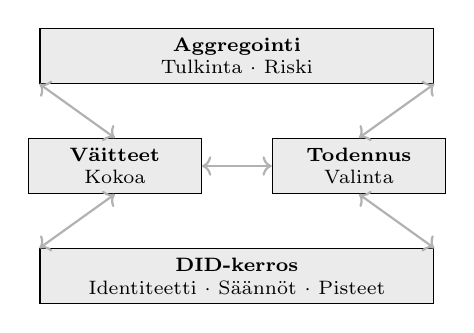
\begin{tikzpicture}[
    layer/.style={draw, minimum height=0.7cm, align=center, font=\scriptsize, fill=black!8},
    arr/.style={<->, thick, gray!60}
]
\node[layer, minimum width=5cm] (agg) at (0,2.8) {\textbf{Aggregointi}\\Tulkinta\ $\cdot$ Riski};
\node[layer, minimum width=2.2cm] (claim) at (-1.55,1.4) {\textbf{Väitteet}\\Kokoa};
\node[layer, minimum width=2.2cm] (verif) at (1.55,1.4) {\textbf{Todennus}\\Valinta};
\node[layer, minimum width=5cm] (did) at (0,0) {\textbf{DID-kerros}\\Identiteetti $\cdot$ Säännöt $\cdot$ Pisteet};

\draw[arr] (agg.south west) -- (claim.north);
\draw[arr] (agg.south east) -- (verif.north);
\draw[arr] (claim.east) -- (verif.west);
\draw[arr] (claim.south) -- (did.north west);
\draw[arr] (verif.south) -- (did.north east);
\end{tikzpicture}
\caption{RSN:n nelikerroksinen arkkitehtuuri.}
\label{fig:architecture}
\end{figure}

\subsection{Osallistujien roolit}

Todennustapahtumaan osallistuu enintään kuusi erillistä DID-roolia (kuva~\ref{fig:roles}): \textbf{Antaja} ($DID_I$, luo ja lähettää väitteen), \textbf{Kohde} ($DID_S$, DID, jota väite koskee---voi olla sama kuin Antaja), \textbf{Auktoriteetti} ($DID_A$, hyväksyy väitteen maksua vastaan; voi myös tarjota todistajapalveluja---\emph{valinnainen}), \textbf{Todistaja} ($DID_{W_{1..n}}$, incognito-valvoja todentajan rehellisyydelle haastekoodien avulla---\emph{valinnainen}), \textbf{Todentaja} ($DID_V$, algoritmisesti valittu julkaisemaan väite) ja \textbf{RSN} (verkosto, jossa todennetut väitteet julkaistaan). Mikä tahansa rooli voidaan delegoida toiselle DID:ille (luku~7.4). Auktoriteetti niputtaa yleisesti hyväksynnän todistajapalveluihin, mutta nämä kaksi tehtävää ovat loogisesti riippumattomia.

\begin{figure}[ht]
\centering
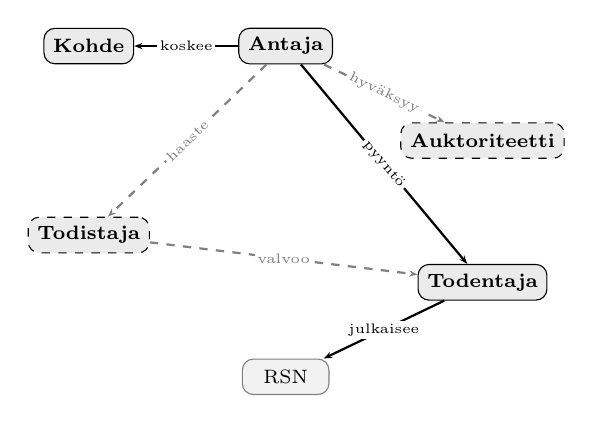
\begin{tikzpicture}[
    role/.style={draw, rounded corners, minimum width=1.1cm, minimum height=0.45cm, align=center, font=\scriptsize, fill=black!8},
    opt/.style={draw, rounded corners, minimum width=1.1cm, minimum height=0.45cm, align=center, font=\scriptsize, fill=black!8, dashed},
    arr/.style={-{Stealth[length=3pt]}, thick},
    oarr/.style={-{Stealth[length=3pt]}, thick, dashed, gray},
    lbl/.style={font=\tiny, fill=white, inner sep=1pt}
]
\node[role] (I) at (0,2.4) {\textbf{Antaja}};
\node[role] (S) at (-2.5,2.4) {\textbf{Kohde}};
\node[opt] (A) at (2.5,1.2) {\textbf{Auktoriteetti}};
\node[opt] (W) at (-2.5,0) {\textbf{Todistaja}};
\node[role] (V) at (2.5,-0.6) {\textbf{Todentaja}};
\node[role, fill=black!5, draw=gray] (N) at (0,-1.8) {RSN};

\draw[arr] (I) -- node[lbl] {koskee} (S);
\draw[oarr] (I) -- node[lbl,sloped] {hyväksyy} (A);
\draw[oarr] (I) -- node[lbl,sloped] {haaste} (W);
\draw[arr] (I) -- node[lbl,sloped] {pyyntö} (V);
\draw[oarr] (W) -- node[lbl] {valvoo} (V);
\draw[arr] (V) -- node[lbl] {julkaisee} (N);
\end{tikzpicture}
\caption{DID-roolit todennustapahtumassa. Katkoviiva = valinnainen (Auktoriteetti, Todistaja).}
\label{fig:roles}
\end{figure}

\subsection{Korruptoitumattomuus: neljä voimaa}

RSN:n korruptoitumattomuus ei synny yksittäisestä mekanismista vaan neljästä samanaikaisesta voimasta. Mikään niistä ei riitä yksinään; vasta niiden yhdistelmä tekee korruptioyrityksestä taloudellisesti irrationaalisen.

\textbf{Ennakoimaton kohde.} Kunkin väitteen todentaja valitaan epädeterministisesti johdonmukaisen tiivistämisen avulla (luku~5.3). Hyökkääjä ei voi kohdentaa lahjontaa ennalta tiettyyn todentajaan, koska todentajan henkilöllisyys on väitteen sisällön ja aiempien iteraatioiden funktio, ei antajan valinnan.

\textbf{Maineen vipuvaikutus---hidas ylös, nopea alas.} Mainetta voi kartuttaa vain vähitellen, jatkuvan johdonmukaisen käyttäytymisen kautta. Se voidaan kuitenkin menettää katastrofaalisesti yhdellä petollisella hyväksynnällä (luku~6.2). Tämä epäsymmetria tarkoittaa, että vuosien kertynyt maine voidaan tuhota yhdellä epärehellisellä hyväksynnällä; optimaalinen strategia on aina hylätä epäilyttävät väitteet.

\textbf{Julkinen lupaus.} Jokainen DID:in haltija ilmoittaa julkisesti käytäntönsä---koneluettavan sääntöjoukon, jota hän sitoutuu noudattamaan. Ilmoituksen ja todellisen käyttäytymisen välinen poikkeama on havaittavissa ja hinnoitellaan mainerikkomukseksi, joka on ankarampi kuin itse taustalla oleva rikkomus (luku~7.3). Tekopyhyys on siten kalliimpaa kuin suora epärehellisyys.

\textbf{Verkkorakenteen hyökkäyskustannuksen epäsymmetria.} Verkoston sensuroinnin tai horjuttamisen kustannus kasvaa epälineaarisesti verkoston koon ja tiheyden mukana, kun taas sen sietämisen kustannus pysyy vakiona. Jotta sensuuri kannattaisi, keskitetyn toimijan olisi sovellettava sitä koko verkostoon---mikä vaatisi toimenpiteitä, jotka ovat suhteettomia mihinkään kuviteltavissa olevaan hyötyyn nähden (luku~10).

% ============================================================
% 4. DECENTRALIZED IDENTITY MODEL
% ============================================================
\section{Hajautetun identiteetin malli}

\subsection{DID erityisominaisuuksin}

RSN laajentaa W3C DID Core -spesifikaatiota~\cite{did2022} seuraavilla: \textbf{Ilmoitetut säännöt} (koneluettavat käyttäytymissitoumukset), \textbf{Mainemetadata} (aggregoitu käyttäytymispistemäärä) ja \textbf{Verkostoreititys} (muuttuva onion-yhdyskäytävä, joka on erillinen vakaasta rengaspositiosta).

\subsection{Väitteen elinkaari}

Väite etenee kuuden vaiheen läpi (kuva~\ref{fig:lifecycle}): kokoaminen, valinnainen auktoriteetin hyväksyntä, todentajan valinta johdonmukaisen tiivistämisen avulla, todennuspäätös (hyväksyntä tai hylkäys iteraatiolla), julkaisu ja maineen päivitys kaikille osapuolille.

\begin{figure}[ht]
\centering
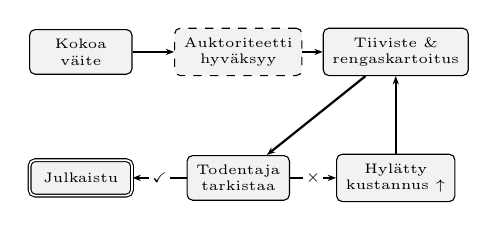
\begin{tikzpicture}[
    stp/.style={draw, rounded corners=2pt, minimum width=1.3cm, minimum height=0.45cm, align=center, font=\tiny, fill=black!5},
    arr/.style={-{Stealth[length=3pt]}, thick},
    lbl/.style={font=\tiny, fill=white, inner sep=1pt}
]
\node[stp] (comp) at (0,0) {Kokoa\\väite};
\node[stp, dashed] (auth) at (2.0,0) {Auktoriteetti\\hyväksyy};
\node[stp] (hash) at (4.0,0) {Tiiviste \&\\rengaskartoitus};
\node[stp] (ver) at (2.0,-1.6) {Todentaja\\tarkistaa};
\node[stp, double] (pub) at (0,-1.6) {Julkaistu};
\node[stp] (rej) at (4.0,-1.6) {Hylätty\\kustannus $\uparrow$};

\draw[arr] (comp) -- (auth);
\draw[arr] (auth) -- (hash);
\draw[arr] (hash) -- (ver);
\draw[arr] (ver) -- node[lbl] {\checkmark} (pub);
\draw[arr] (ver) -- node[lbl] {$\times$} (rej);
\draw[arr] (rej) -- ++(0,0.8) -| (hash);
\end{tikzpicture}
\caption{Väitteen elinkaari iteraatiosilmukalla.}
\label{fig:lifecycle}
\end{figure}

\subsection{Suhde W3C DID Core -spesifikaatioon}

RSN:n identiteettimalli on W3C DID Core -spesifikaation~\cite{did2022} varsinainen ylijoukko. Kaikki RSN-DID:t ovat päteviä W3C-DID:ejä. RSN:lle ominaiset laajennukset koodataan DID-dokumentin ominaisuuksina, jotka määritellään omistetussa DID-menetelmäspesifikaatiossa, yhteensopivana olemassa olevan infrastruktuurin kuten ION:in~\cite{buchner2021} ja Ceramicin~\cite{ceramic2023} kanssa.

% ============================================================
% 5. VERIFICATION AND PROPAGATION
% ============================================================
\section{Tiedon todentaminen ja leviäminen}

\subsection{Tiedon syöttämisen kustannus}

RSN:n taloudellinen ydinperiaate on lukemisen ja kirjoittamisen välinen epäsymmetria. Mainetiedon lukeminen lähestyy nollaa rajakustannusta osallistujille, jotka ovat osa DID-verkostoa ja joilla on maineensa mukainen pääsy---tulokkaiden on ansaittava laajempi pääsy vähitellen (ks. loisimisen esto). Kirjoittaminen---ymmärrettynä maineen kestävänä konkretisoitumisena verkostoon, ei yksittäisenä teknisenä toimena---vaatii todennettavaa kumulatiivista panostusta kolmella ulottuvuudella: \textbf{aika} (elinvuodet, jotka on käytetty johdonmukaiseen käyttäytymiseen, täytettyihin sitoumuksiin ja vaalittuihin suhteisiin), \textbf{energia} (rehelliseen toimintaan, kumppanuuksien vaalimiseen ja pitkäaikaiseen luotettavuuteen sijoitettu ponnistus) ja \textbf{raha} (sijoitus omaan nimeen---ammatillinen kehittyminen, oman työn laatu, aiheutettujen vahinkojen hyvittäminen). Mainetta ei voi ostaa hetkessä---se on elinikäisen kertymän lopputulos, jonka järjestelmä vain tekee näkyväksi ja siirrettäväksi kontekstien välillä. Protokollan kertaluonteiset tekniset kustannukset (kryptografiset allekirjoitukset, todentajan maksut) ovat mitättömiä tähän taustalla olevaan sijoitukseen verrattuna.

\subsection{Sosiaalinen graafi ja kontaktien syvyys}

RSN on pohjimmiltaan sosiaalinen verkosto: kukin DID lisää kontakteja (muita DID:ejä), jotka sallivat yhteyden. Näillä kontakteilla on omat kontaktinsa, ja niin edelleen. Algoritminen todentajan haku toimii säädettävän linkitettyjen kontaktien syvyyden $h$ sisällä (esim. $h=3$: omat suorat kontaktit, heidän kontaktinsa ja kontaktien kontaktit). Tämä arkkitehtuuri ei vaadi yhtä globaalia lohkoketjua---se suosii luonnostaan yhteisöjen/klustereiden syntymistä, jotka limittyvät muihin yhteisöihin. Jokaisella DID-osallistujalla on oltava julkaistu \textbf{käytäntö}---koneluettava sääntöjoukko, joka ohjaa saapuvien pyyntöjen arviointia. Käytäntörikkomukset kirjataan verkostoon negatiivisina artefakteina.

\subsection{Algoritminen todentajan valinta}

Todennusprotokolla käyttää johdonmukaista tiivistämistä~\cite{karger1997} (kuva~\ref{fig:verifier}). Todentaminen on maksullinen palvelu: todentajat toimivat maksua vastaan, mikä luo markkinat, joissa kilpailu ohjaa hinnoittelua, nopeutta ja luotettavuutta.

\textbf{Vaihe 1.} Väitedokumentti ketjutetaan edellisen iteraation tiivistetulokseen (tai $\varnothing$ ensimmäisellä iteraatiolla) ja tiivistetään:
\begin{equation}
\text{pos} = f_h(\text{väite} \| \text{prev\_hash})
\label{eq:hash}
\end{equation}

Algoritmin on sisällettävä kaikkien aiempien pyyntöjen ja vastausten \emph{täydellinen polku}---ei pelkkää edellisen iteraation tiivistettä. Kunkin todentajan koko vastaus (hyväksyntä, hylkäys, ilmoitettu hinta, perustelu) liitetään kasvavaan dokumenttiin, todennettavana kryptografisten allekirjoitusten avulla joka vaiheessa.

\textbf{Vaihe 2.} Tiiviste kartoitetaan $N$ positioon johdonmukaisen tiivistysrenkaan ympärille, tasaisesti jaettuina (esim. $N=4$: $+0^{\circ}, +90^{\circ}, +180^{\circ}, +270^{\circ}$). Kustakin positiosta myötäpäivään suuntautuva haku valitsee lähimmän DID:in todentajaehdokkaaksi (kuva~\ref{fig:multipoint}). $N$ on muuttuva parametri, joka voi riippua parhaillaan aktiivisten DID:ien prosenttiosuudesta, vuorokaudenajasta tai verkoston historiallisesta vasteajasta.

\textbf{Vaihe 3.} Todentaja hyväksyy (julkaisee, panttaa maineensa) tai hylkää (palaa vaiheeseen~1 hylkäystiivisteen kanssa). Kun solmu ei vastaa, vaikka se ilmoittaa olevansa verkossa, seuraavan pyynnön on sisällettävä kaikki vastaukset kaikilta $N$ aiemmalta todentajaehdokkaalta.

\textbf{Loisimisen esto.} Kohde-DID:t voivat asettaa maksuja tai pääsyrajoituksia kyselyille vähän mainetta omaavilta uusilta DID:eiltä. Tämä porrastettu mekanismi (ei binäärinen) pakottaa tulokkaat rakentamaan mainetta aidon toiminnan kautta ennen kuin he saavat vapaasti kuluttaa muiden dataa.

\begin{figure}[ht]
\centering
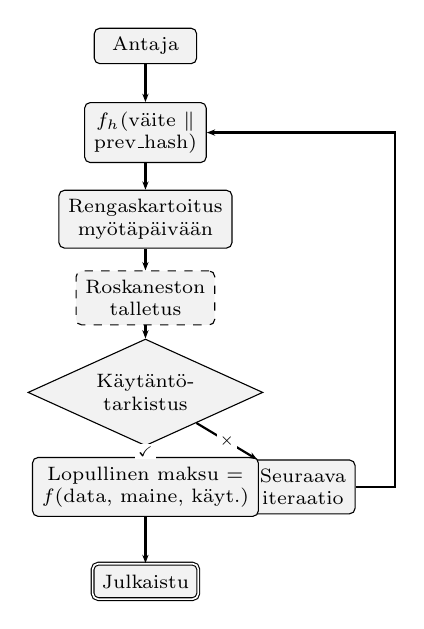
\begin{tikzpicture}[
    box/.style={draw, rounded corners=2pt, minimum width=1.3cm, minimum height=0.45cm, align=center, font=\scriptsize, fill=black!5},
    dec/.style={draw, diamond, aspect=2.2, minimum width=0.9cm, align=center, font=\scriptsize, fill=black!5},
    arr/.style={-{Stealth[length=3pt]}, thick},
    lbl/.style={font=\tiny, fill=white, inner sep=1pt}
]
\node[box] (iss) at (0,0) {Antaja};
\node[box] (hash) at (0,-1.1) {$f_h$(väite $\|$\\prev\_hash)};
\node[box] (ring) at (0,-2.2) {Rengaskartoitus\\myötäpäivään};
\node[box, dashed] (spam) at (0,-3.2) {Roskaneston\\talletus};
\node[dec] (check) at (0,-4.4) {Käytäntö-\\tarkistus};
\node[box] (rej) at (2,-5.6) {Seuraava\\iteraatio};
\node[box] (fee) at (0,-5.6) {Lopullinen maksu =\\$f$(data, maine, käyt.)};
\node[box, double] (pub) at (0,-6.8) {Julkaistu};

\draw[arr] (iss) -- (hash);
\draw[arr] (hash) -- (ring);
\draw[arr] (ring) -- (spam);
\draw[arr] (spam) -- (check);
\draw[arr] (check) -- node[lbl] {$\times$} (rej);
\draw[arr] (check) -- node[lbl] {\checkmark} (fee);
\draw[arr] (fee) -- (pub);
\draw[arr] (rej.east) -- ++(0.5,0) |- (hash.east);
\end{tikzpicture}
\caption{Todentajan valintaprotokolla. Roskaneston talletus on valinnainen ja voi olla palautettavissa. Lopullinen maksu maksetaan vain hyväksynnän yhteydessä.}
\label{fig:verifier}
\end{figure}

Kukin hylkäys liittää todentajan koko vastauksen (mukaan lukien perustelut ja ehdot) väitedokumenttiin, laajentaen sen sisältöä. Laajennetusta dokumentista lasketaan epädeterministisesti uusi tiiviste, joka kartoittuu eri rengaspositioon ja valitsee eri todentajan. Koko polun dokumentointi on pakollista---antaja ei voi ennustaa tai vaikuttaa seuraavaan todentajaan. Jos todentaja jättää pyynnön huomiotta yhteensopivasta ilmoitetusta käytännöstä huolimatta, todistajat (jos läsnä) kirjaavat tämän, ja antaja voi liittää todistajien todisteet lopulliseen julkaisuun.

\begin{figure}[ht]
\centering
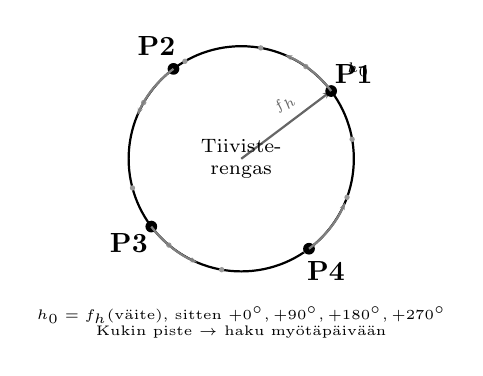
\begin{tikzpicture}[scale=0.65]
% Ring
\draw[thick] (0,0) circle (2.2cm);
% DID nodes on ring
\foreach \a in {10,55,80,120,150,195,230,260,305,340} {
  \fill[black!40] (\a:2.2) circle (1.5pt);
}
% Hash offset arrow pointing to initial position
\draw[-{Stealth[length=3pt]}, thick, black!60] (0,0) -- node[font=\tiny,above,sloped,pos=0.6] {$f_h$} (37:2.2);
\fill[black] (37:2.2) circle (2pt);
\node[font=\tiny,anchor=south west] at (37:2.35) {$h_0$};
% N=4 points offset from h0 by +0, +90, +180, +270
\foreach \offset/\l in {0/P1,90/P2,180/P3,270/P4} {
  \pgfmathsetmacro{\ang}{37+\offset}
  \node[fill=black, circle, inner sep=1.5pt] (p\offset) at (\ang:2.2) {};
  \node[font=\tiny,font=\bfseries] at (\ang:2.75) {\l};
  % clockwise search arc
  \draw[-{Stealth[length=2.5pt]}, thick, gray] (\ang:2.2) arc (\ang:\ang+30:2.2);
}
\node[font=\scriptsize, align=center] at (0,0) {Tiiviste-\\rengas};
\node[font=\tiny, align=center] at (0,-3.2) {$h_0 = f_h(\text{väite})$, sitten $+0^{\circ},+90^{\circ},+180^{\circ},+270^{\circ}$\\Kukin piste $\rightarrow$ haku myötäpäivään};
\end{tikzpicture}
\caption{Monipistevalinta ($N{=}4$). Tiiviste $h_0$ asettaa siirtymän; 4 pistettä tasaisesti jaettuina $h_0$:sta.}
\label{fig:multipoint}
\end{figure}

\subsection{Todistajaprotokolla}

\textbf{Todistaja}-rooli tarjoaa incognito-vastuuvelvollisuuden todentajan rehellisyydelle kryptografisen haastekoodiprotokollan kautta:

\textbf{Vaihe W1.} Pyytäjä allekirjoittaa todennuspyynnön ja lähettää sen $N_w$ todistajalle---kontakteille pyytäjän sosiaalisesta verkostosta tai maksua vastaan toimiville erikoistuneille todistajapalvelun tarjoajille.

\textbf{Vaihe W2.} Kukin todistaja $w_i$ allekirjoittaa koko allekirjoitetun pyynnön, säilyttää alkuperäisen allekirjoituksen $\sigma_i$ ja laskee haastekoodin $c_i = h(\sigma_i)$. Haastekoodi liitetään pyyntöön.

\textbf{Vaihe W3.} Pyyntö, joka nyt kantaa $N_w$ haastekoodia, lähetetään todentajalle. Todentaja näkee koodit mutta \emph{ei voi määrittää}, keitä todistajat ovat tai vastaavatko koodit todellisia allekirjoituksia.

\textbf{Vaihe W4 (rehellinen todentaja).} Jos todentaja vastaa ilmoittamansa käytännön mukaisesti, haastekoodit pysyvät läpinäkymättöminä. Todistajia ei koskaan paljasteta. Lisädataa ei julkaista.

\textbf{Vaihe W5 (käytäntörikkomus).} Jos todentaja rikkoo käytäntöään (jättää pyynnön huomiotta, vastaa epäjohdonmukaisesti), pyytäjällä on hallussaan todistajien alkuperäiset allekirjoitukset $\sigma_i$. Nämä voidaan julkaista oheisdatana: kuka tahansa voi todentaa $c_i = h(\sigma_i)$, mikä todistaa todistajan olleen läsnä. Pyytäjä voi julkaista itsenäisesti---todentaja allekirjoitti haastekoodit jo vastauksessaan.

\textbf{Bluffiominaisuus.} Pyytäjä voi korvata osan tai kaikki haastekoodit satunnaisilla arvoilla. Todentaja ei voi erottaa aitoja koodeja (korkean maineen auktoriteettien tukemia) kohinasta. Tämä \emph{epävarmuus} on täytäntöönpanomekanismi: jokainen pyyntö kantaa riskin siitä, että arvostettu auktoriteetti seuraa incognito. Tämän paineen ylläpitämisen kustannus on lähes nolla (satunnaislukujen generointi), kun taas epärehellisyyden mahdollinen kustannus todentajalle on katastrofaalinen. Rehelliseen käyttäytymiseen kannustetaan, vaikka todellisia todistajia ei olisikaan.

\textbf{Auktoriteetti todistajana.} Auktoriteetti, joka hyväksyy väitteen, voi niputtaa mukaan todistajapalveluja: ``Hyväksyn väitteesi ja toimin incognito-todistajana todennuksen aikana.'' Tämä on luonnollinen liiketoimintamalli---auktoriteetilla on jo konteksti. Nämä kaksi roolia ovat kuitenkin loogisesti riippumattomia.

\subsection{Kalliin radikalismin periaate}

Kolme kustannuskanavaa kasautuvat samanaikaisesti (kuva~\ref{fig:radicalism}):

\textbf{Kanava 1: Iteraatiokustannus.} Kukin hylkäys pakottaa uuteen iteraatioon, joka kuluttaa aikaa ja resursseja. Lineaarinen kasvu.

\textbf{Kanava 2: Dokumentin paisuminen.} Kukin iteraatio lisää todentajan koko vastauksen väitedokumenttiin. Kasvu on lineaarista, mutta perussiirtymällä: alkuperäisellä hyötykuormalla (väitteen sisältö, auktoriteetin hyväksyntä, kryptografiset allekirjoitukset) on jo ei-triviaali koko $B_0$. Kokonaiskoko $k$ iteraation jälkeen: $S(k) = B_0 + k \cdot \Delta$, missä $\Delta$ on keskimääräinen vastauksen koko.

\textbf{Kanava 3: Todentajan riskilisä.} Riski on subjektiivinen. Todentaja arvioi, ovatko pyytävän DID:in ilmoitetut käytännöt ristiriidassa todentajan omien kaupallisten, sosiaalisten tai poliittisten etujen kanssa. Lisä voi kasvaa eksponentiaalisesti havaitun etäisyyden mukaan todentajan ``ihanteesta'': $P(d) = \alpha \cdot e^{\beta d}$, missä $d$ on todentajan subjektiivinen etäisyysmitta. Henkilökohtaisen ehdottoman rajan ylittyessä todentaja voi kieltäytyä kokonaan.

\begin{figure}[ht]
\centering
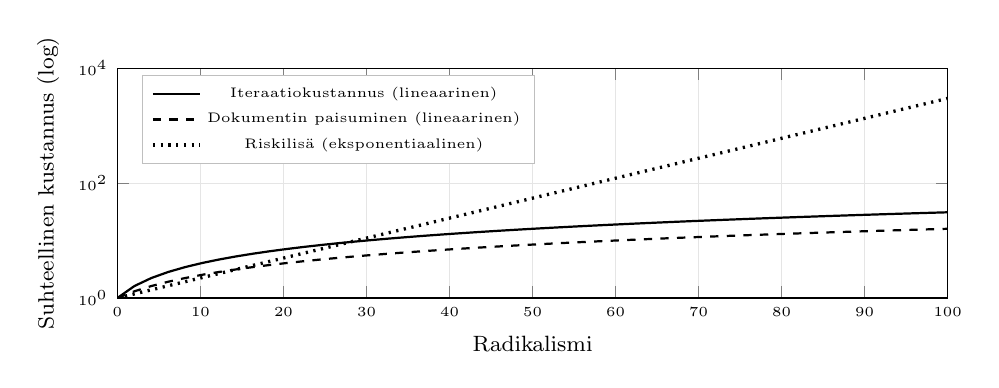
\begin{tikzpicture}
\begin{axis}[
    width=\columnwidth,
    height=4.5cm,
    xlabel={\footnotesize Radikalismi},
    ylabel={\footnotesize Suhteellinen kustannus (log)},
    ymode=log,
    xmin=0, xmax=100,
    ymin=1, ymax=10000,
    grid=major,
    grid style={gray!20},
    legend style={at={(0.03,0.97)},anchor=north west,font=\tiny,draw=gray!50},
    tick label style={font=\tiny},
    label style={font=\footnotesize},
]
\addplot[black, thick, domain=0:100, samples=50] {1 + 0.3*x};
\addlegendentry{Iteraatiokustannus (lineaarinen)}
\addplot[black, thick, dashed, domain=0:100, samples=50] {1 + 0.15*x};
\addlegendentry{Dokumentin paisuminen (lineaarinen)}
\addplot[black, thick, dotted, line width=1.2pt, domain=0:100, samples=100] {exp(0.08*x)};
\addlegendentry{Riskilisä (eksponentiaalinen)}
\end{axis}
\end{tikzpicture}
\caption{Kustannusten kärjistyminen kolmessa kanavassa. Riskilisä hallitsee korkealla radikalismilla.}
\label{fig:radicalism}
\end{figure}

Ratkaisevasti tämä ei ole sensuuria. Mitään väitettä ei kielletä. Järjestelmä hinnoittelee riskin (taulukko~\ref{tab:costs}).

\begin{table}[ht]
\centering
\caption{Kustannusvertailu väitetyyppien välillä.}
\label{tab:costs}
\footnotesize
\begin{tabular}{@{}lcccc@{}}
\toprule
\textbf{Tyyppi} & \textbf{Iter.} & \textbf{Dok.} & \textbf{Maksu} & \textbf{Yht.} \\
\midrule
Uskottava & $k_{\min}$ & $B_0$ & $P_{\min}$ & Matala \\
Kiistanalainen & $k_{\text{med}}$ & $B_0{+}k\Delta$ & $\alpha e^{\beta d}$ & Kohtalainen \\
Radikaali & $k_{\max}$ & $\gg B_0$ & $\gg P_{\min}$ & Erittäin korkea \\
Petollinen & $\to\infty$ & --- & --- & Julkaisukelvoton \\
\bottomrule
\end{tabular}
\end{table}

% ============================================================
% 6. REPUTATION AND RISK
% ============================================================
\section{Maine ja riskinarviointi}

\subsection{Maineen kertymämalli}

Maineella on kolme ominaisuutta: \textbf{hidas kertyminen} (asteittainen kasvu johdonmukaisen käyttäytymisen kautta), \textbf{nopea tuhoutuminen} (yksi petos voi laskea pistemäärää katastrofaalisesti) ja \textbf{yksilöllinen arviointi} (kukin kuluttava osapuoli voi soveltaa omaa aggregointifunktiotaan).

\subsection{Maineikkaat auktoriteetit}

Maineikas auktoriteetti tarkastaa väitteet ja, jos on tyytyväinen, allekirjoittaa ne yhdessä---pantaten oman maineensa (kuva~\ref{fig:authority}). Epäsymmetria on tarkoituksellinen: maineen ansaitseminen on hidasta (asteittainen $+\delta$ kutakin rehellistä hyväksyntää kohti), kun taas sen menettäminen on katastrofaalista ($-\Delta \gg \delta$ kutakin väärää hyväksyntää kohti; havainnollistavasti esim. $+2\%$ vs.\ $-70\%$). Optimaalinen strategia on aina hylätä epäilyttävät väitteet. Arvojen $\delta$ ja $\Delta$ tarkat arvot ovat järjestelmäparametreja.

\begin{figure}[ht]
\centering
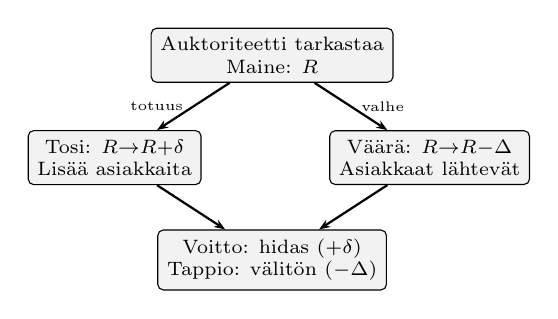
\begin{tikzpicture}[
    box/.style={draw, rounded corners=2pt, minimum width=2cm, minimum height=0.6cm, align=center, font=\scriptsize, fill=black!5},
    arr/.style={-{Stealth[length=4pt]}, thick}
]
\node[box] (exam) at (0,0) {Auktoriteetti tarkastaa\\Maine: $R$};
\node[box] (true) at (-2,-1.3) {Tosi: $R{\to}R{+}\delta$\\Lisää asiakkaita};
\node[box] (false) at (2,-1.3) {Väärä: $R{\to}R{-}\Delta$\\Asiakkaat lähtevät};
\node[box] (insight) at (0,-2.6) {Voitto: hidas ($+\delta$)\\Tappio: välitön ($-\Delta$)};

\draw[arr] (exam) -- node[left,font=\tiny] {totuus} (true);
\draw[arr] (exam) -- node[right,font=\tiny] {valhe} (false);
\draw[arr] (true) -- (insight);
\draw[arr] (false) -- (insight);
\end{tikzpicture}
\caption{Maineikas auktoriteetti---epäsymmetriset kannustimet.}
\label{fig:authority}
\end{figure}

\subsection{Moniulotteinen maine}

Maine ei ole skalaari vaan vektori useiden ulottuvuuksien yli: taloudellinen luotettavuus, henkilökohtainen rehellisyys, ammatillinen pätevyys, kansalaisosallistuminen ja muut (kuva~\ref{fig:reputation-radar}). Eri arviointipalvelut projisoivat tämän vektorin eri tavoin kontekstista riippuen---lainanantaja priorisoi taloudellista luotettavuutta, työnantaja ammatillista pätevyyttä, naapuri kansalaiskäyttäytymistä. Ei ole yhtä ``oikeaa'' mainepistemäärää; vain näkökulmia.

\begin{figure}[ht]
\centering
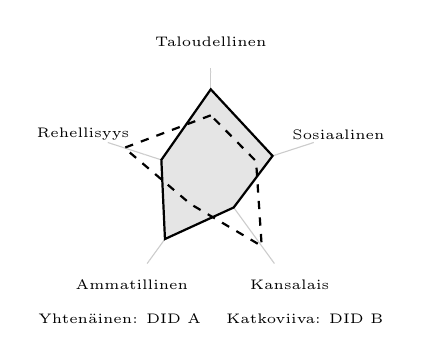
\begin{tikzpicture}[scale=0.55]
\foreach \a/\l in {90/Taloudellinen,162/Rehellisyys,234/Ammatillinen,306/Kansalais,18/Sosiaalinen} {
  \draw[gray!40] (0,0) -- (\a:2.5);
  \node[font=\tiny, align=center] at (\a:3.1) {\l};
  \foreach \r in {0.8,1.6,2.4} {
    \fill[black!15] (\a:\r) circle (0.5pt);
  }
}
\draw[thick, fill=black!10] (90:2.0) -- (162:1.2) -- (234:1.8) -- (306:0.9) -- (18:1.5) -- cycle;
\draw[thick, dashed] (90:1.4) -- (162:2.1) -- (234:0.8) -- (306:2.0) -- (18:1.1) -- cycle;
\node[font=\tiny] at (0,-3.3) {Yhtenäinen: DID A \quad Katkoviiva: DID B};
\end{tikzpicture}
\caption{Moniulotteiset mainevektorit. Eri DID:t osoittavat erilaisia profiileja ulottuvuuksien yli.}
\label{fig:reputation-radar}
\end{figure}

\subsection{Demokratisoitu riskinarviointi}

RSN demokratisoi järjestelmällisen riskinarvioinnin---kyvyn, joka on tällä hetkellä keskittynyt rahoituslaitoksiin mutta soveltuu paljon pankkitoimintaa laajemmalle. Teollisuuskonglomeraatit arvioimassa toimittajien luotettavuutta, vakuutusyhtiöt hinnoittelemassa käyttäytymisriskiä, due diligence yrityskaupoissa ja -sulautumisissa, laitteiden eliniän arviointi valmistuksessa---missä tahansa vastapuoliriski vaatii arviointia, RSN tarjoaa hajautetun, markkinavetoisen vaihtoehdon. Tulkintapalveluiden markkinat kääntävät raa'an moniulotteisen mainedatan toimintakelpoisiksi yhteenvedoiksi, tehden vastapuolen arvioinnista minkä tahansa osallistujan saatavilla olevaa rajakustannuksin.

% ============================================================
% 7. CONSENSUS AND DISPUTE RESOLUTION
% ============================================================
\section{Konsensus ja riitojenratkaisu}

\subsection{Hajautetun oikeuden malli}

RSN muotoilee oikeuden uudelleen kaksisuuntaisena neuvotteluongelmana. Pysyvän, todennettavan mainevahingon uhka on tehokkaampi pelote kuin oikeudenkäynti, johon vahinkoa kärsinyt osapuoli ei ole varaa.

\subsection{Emergentti konsensus}

Kukin osallistuja ylläpitää henkilökohtaista tyytyväisyyskynnystä. Verkoston kokonaiskonsensus syntyy tuhansien kaksisuuntaisten neuvottelujen tilastollisena keskiarvona (kuva~\ref{fig:consensus}). Konsensuksen kaukana yläpuolella oleva vastaus (barbaarinen) on kallis julkaista. Konsensuksen lähellä oleva vastaus (suhteellinen) on halpa. Konsensus ei ole sääntö---se on hintasignaali.

\begin{figure}[ht]
\centering
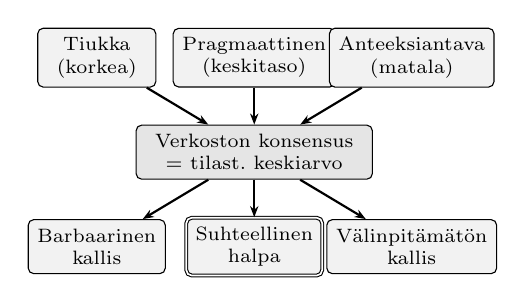
\begin{tikzpicture}[
    person/.style={draw, rounded corners=2pt, minimum width=1.5cm, minimum height=0.5cm, align=center, font=\scriptsize, fill=black!5},
    arr/.style={-{Stealth[length=4pt]}, thick}
]
\node[person] (a) at (-2,0) {Tiukka\\(korkea)};
\node[person] (b) at (0,0) {Pragmaattinen\\(keskitaso)};
\node[person] (c) at (2,0) {Anteeksiantava\\(matala)};
\node[person, fill=black!10, minimum width=3cm] (cons) at (0,-1.2) {Verkoston konsensus\\= tilast.\ keskiarvo};
\node[person] (exp) at (-2,-2.4) {Barbaarinen\\kallis};
\node[person, double] (prop) at (0,-2.4) {Suhteellinen\\halpa};
\node[person] (neg) at (2,-2.4) {Välinpitämätön\\kallis};

\draw[arr] (a) -- (cons);
\draw[arr] (b) -- (cons);
\draw[arr] (c) -- (cons);
\draw[arr] (cons) -- (exp);
\draw[arr] (cons) -- (prop);
\draw[arr] (cons) -- (neg);
\end{tikzpicture}
\caption{Emergentti konsensus yksilöllisistä tyytyväisyyskynnyksistä.}
\label{fig:consensus}
\end{figure}

\subsection{Rangaistuksen kalibrointi}

Kukin DID:in haltija ilmoittaa julkisesti vastauksensa tiettyihin väärinkäytöskategorioihin. Suhteettoman ankarat tai lempeät ilmoitukset houkuttelevat negatiivisia mainesignaaleja. Suhteelliset ilmoitukset hyväksytään kitkatta---itseään kalibroiva rangaistusjärjestelmä.

Konsensusilmoitukset ovat itsessään tekopyhyyden havaitsemisen alaisia: konsensuskantaan sitoutuminen julistuksen tasolla samalla epäjohdonmukaisesti käyttäytyen muodostaa mainerikkomuksen, joka on ankarampi kuin taustalla oleva poikkeama, koska se osoittaa tahallista petosta.

\subsection{Delegointi}

Kaikki DID:in sisäiset toiminnot---yhtä poikkeusta lukuun ottamatta---voidaan delegoida toiselle DID:ille. \textbf{Kohde-roolia---DID:iä, jonka käyttäytymistä väite koskee---ei voi delegoida; se on siirtokelvottomasti sidottu siihen identiteetin haltijaan, johon väite viittaa.} Muut aktiiviset roolit---Antaja, Auktoriteetti, Todistaja, Todentaja---voidaan siirtää nimetylle valtuutetulle DID:ille, olipa kyse todennuksesta, väitteen lähettämisestä, konsensukseen osallistumisesta tai riitojenratkaisusta. Delegointi on peruutettavissa milloin tahansa. Tämä mahdollistaa erikoistumisen (esim. ammattimaiset todennuspalvelut), samalla kun haltija säilyttää perimmäisen hallinnan ja vastuun. Delegointi koskee koko järjestelmää ja on olennaista skaalautuvuudelle.

\subsection{Yksilön moraalista emergenttiin yhteiskuntasopimukseen}

Kunkin DID:in ilmoitettu käytäntö edustaa yksilön moraalin formalisointia: mitä haltija pitää hyväksyttävänä, miten hän vastaa tiettyihin käyttäytymisiin, mitä hän vaatii vastapuolilta. Näitä käytäntöjä ei aseta järjestelmän suunnittelija---kukin osallistuja valitsee ne ja ilmaisee koneluettavassa muodossa.

Tämä formalisointi mahdollistaa kolmivaiheisen emergenssin. Ensin yksilön moraali koodataan \textbf{käytännöksi}---joukoksi ilmoitettuja sääntöjä, kynnyksiä ja vastefunktioita, joita DID sitoutuu noudattamaan. Toiseksi kaikkien verkoston käytäntöjen kokonaisuus tuottaa \textbf{emergentin etiikan}---tilastollisesti havaittavia normeja, joita yksikään osallistuja ei suunnitellut mutta jotka syntyvät tuhansien yksilöllisten moraalikantojen vuorovaikutuksesta~\cite{durkheim1893}. Kolmanneksi tämä emergentti etiikka, ilmaistuna jaettuina käyttäytymisnormeina, joita valvotaan kaksisuuntaisilla hintasignaaleilla, muodostaa \textbf{mitattavissa olevan yhteiskuntasopimuksen}---ei teoreettisen rakennelman, jota kukaan ei allekirjoittanut~\cite{rawls1971}, vaan empiirisesti havaittavan sääntöjoukon, jota todellinen käyttäytyminen tukee.

Tämä prosessi heijastelee moraalisten perustusten teorian löydöksiä~\cite{haidt2012}: inhimillinen moraali on intuitiivinen, pluralistinen ja kulttuurisesti vaihteleva. RSN ei vaadi moraalista konsensusta syötteenä; se tuottaa käyttäytymiskonsensuksen tuloksena. Näin syntyvä yhteiskuntasopimus ei ole staattinen---se kehittyy, kun osallistujat liittyvät, poistuvat ja säätävät käytäntöjään verkoston palautteen mukaan. Toisin kuin klassinen yhteiskuntasopimusteoria, tämä sopimus on peruutettavissa, havaittavissa ja täytäntöönpanokelpoinen ilman suvereenia.

% ============================================================
% 8. ECONOMIC MODEL
% ============================================================
\section{Talousmalli}

Edeltävät luvut kuvasivat työkalua---RSN:n todennusmekanismeja, kustannusrakennetta ja emergenttiä konsensusta. Tämä luku kuvaa metodologiaa tämän työkalun soveltamiseksi finanssi- ja hallintosiirtymään. Työkalu on yleiskäyttöinen; alla oleva metodologia on yksi mahdollinen sovellus.

\subsection{Kannustinrakenne}

Maine pääomana luo suoria kannustimia rehelliseen käyttäytymiseen. Normaalitoiminnassa osallistujat rakentavat mainetta luonnostaan jokapäiväisten transaktioiden ja täytettyjen sitoumusten kautta. Ensisijainen menoerä liittyy \emph{negatiivisiin} väitteisiin---muiden aiheuttaman vahingon kirjaamiseen. Tämä epäsymmetria kannustaa hyödylliseen, luotettavaan käyttäytymiseen: rehellinen oleminen ei maksa ylimääräistä, kun taas vahingollinen oleminen luo dokumentoidun jäljen, jonka muut maksavat säilyttääkseen. Tekopyhyys---sääntöjen ilmoittaminen niitä noudattamatta---on kallein epäonnistumisen muoto, koska se osoittaa tahallista petosta.

\subsection{Rinnakkainen finanssijärjestelmä}

Kolme komponenttia mahdollistaa kilpailullisen paineen: (1)~\textbf{Yksinkertainen vero}---yksi suhteellinen prosentti ilman poikkeuksia, aluksi marginaalisesti nykyisen efektiivisen prosentin alapuolella; (2)~\textbf{Sähköinen menorekisteröinti (Electronic Spending Registration, ESR)}---kääntäen Tšekin EET-mallin niin, että kansalaiset valvovat valtion menoja; (3)~\textbf{Kansalaisohjattu verojen kohdentaminen}---alkaen muutamasta prosentista ensimmäisenä vuonna ja saavuttaen vuosikymmenen jälkeen mitä tahansa alhaisista kaksinumeroisista luvuista täyteen siirtymään kansalaisohjattuun järjestelmään, omaksumisen nopeudesta riippuen. Todellinen tahti riippuu siitä, kuinka nopeasti valtion palveluiden vapaiden markkinoiden vaihtoehtoja syntyy, ja valtion halukkuudesta tehdä yhteistyötä siirtymän kanssa; ajan funktion ei tarvitse olla lineaarinen, eikä ole mitään syytä asettaa ylärajaa sille, mihin omaksuminen voi lopulta yltää.

% ============================================================
% 9. MIGRATION PATH
% ============================================================
\section{Siirtymäpolku}

Siirtymä etenee kolmen vaiheen läpi (kuva~\ref{fig:migration}): \textbf{Vaihe~1: Päällyskerros} (RSN informaatiokerroksena, valtio ainoa tarjoaja), \textbf{Vaihe~2: Kilpailu} (RSN tarjoaa toiminnallisia vaihtoehtoja, kaksoisjärjestelmän käyttö) ja \textbf{Vaihe~3: Siirtymä} (RSN ylittää valtion vastineet, vapaaehtoinen siirtyminen). Siirtymä on peruutettavissa jokaisessa vaiheessa.

\begin{figure}[ht]
\centering
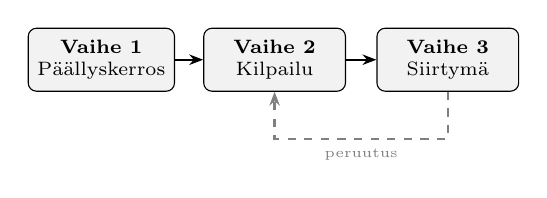
\begin{tikzpicture}[
    phase/.style={draw, rounded corners=3pt, minimum width=1.8cm, minimum height=0.8cm, align=center, font=\scriptsize, fill=black!5},
    arr/.style={-{Stealth[length=5pt]}, thick}
]
\node[phase] (p1) at (0,0) {\textbf{Vaihe 1}\\Päällyskerros};
\node[phase] (p2) at (2.2,0) {\textbf{Vaihe 2}\\Kilpailu};
\node[phase] (p3) at (4.4,0) {\textbf{Vaihe 3}\\Siirtymä};

\draw[arr] (p1) -- (p2);
\draw[arr] (p2) -- (p3);
\draw[arr, dashed, gray] (p3.south) -- ++(0,-0.6) -| node[below,font=\tiny,pos=0.25] {peruutus} (p2.south);
\end{tikzpicture}
\caption{Kolmivaiheinen siirtymä---peruutettavissa jokaisessa vaiheessa.}
\label{fig:migration}
\end{figure}

Ensisijainen painemekanismi on finanssipoliittinen: kun ehdolliset veronmaksajat saavuttavat ``taloudellisesti merkittävän vähemmistön $X$''---ryhmän, joka on kyllin suuri, jotta sitä vastaan kohdistuva sortaminen aiheuttaa ei-triviaalia taloudellista vahinkoa ja kansalaistottelemattomuudesta tulee uskottava uhka---valtio ryhtyy neuvottelemaan. Havainnollistuksen vuoksi käytämme $X \approx 15\%$ BKT:sta, mutta todellinen kynnys riippuu kyseisestä taloudesta.

% ============================================================
% 10. SECURITY ANALYSIS
% ============================================================
\section{Turvallisuusanalyysi}

Tarkastelemme viittä vastustajakategoriaa: yksittäiset pahantekijät, järjestäytyneet ryhmät, yritysvastustajat, valtiotason vastustajat ja protokollatason vastustajat.

\textbf{Sybil-vastustuskyky}~\cite{douceur2002}. Maineen rakentaminen vaatii jatkuvaa, todennettavaa vuorovaikutusta. Onnistuneen Sybil-hyökkäyksen kustannus skaalautuu lineaarisesti valeidentiteettien mukaan ja neliöllisesti kohdemainetason mukaan. Useiden DID:ien käyttäminen rinnakkain on mahdollista mutta suunnittelultaan kallista---kunkin identiteetin on itsenäisesti kartutettava mainetta aidon toiminnan kautta. Vapaissa yhteiskunnissa tämä kustannus ehkäisee satunnaista väärinkäyttöä; diktatuureissa rinnakkaiset DID:t muuttuvat selviytymistyökaluksi, joka mahdollistaa lokeroidun vastarinnan, maanalaisen koordinaation ja turvallisemman mustan pörssin navigoinnin.

\textbf{Salaliittopuolustus.} Suljettujen ryhmien keskinäisen hyväksynnän kuviot ovat havaittavissa sosiaalisen graafin analyysin kautta. Maineen aggregointifunktiot alentavat tiiviisti klusteroituneiden lähteiden väitteitä.

\textbf{Valtiotason vastustaja.} Onion-reititys, keskitetyn infrastruktuurin puuttuminen ja Todentaja-roolin jakautuminen osallistujakannan kesken varmistavat, että tukahduttaminen vaatii toimenpiteitä, jotka ovat suhteettomia mihinkään hyötyyn nähden.

\textbf{Yksityisyys vs.\ vastuuvelvollisuus.} Salanimisyys---välimaasto anonymiteetin ja identiteetin paljastamisen välillä---antaa DID:ien kartuttaa merkityksellistä mainetta paljastamatta haltijan todellisen maailman identiteettiä.

% ============================================================
% 11. PRIVACY
% ============================================================
\section{Yksityisyysnäkökohdat}

RSN:n yksityisyysmalli rakentuu salanimisyydelle. Haltija hallitsee identiteetin paljastamista: minimaalinen (puhdas salanimi), valikoiva (tietyt tunnistetiedot linkitetty) tai täysi (laillinen identiteetti liitetty). Julkaistut väitteet ovat pysyviä---järjestelmä tukee kontekstuaalista korjausta mutta ei poistamista. Haltija voi hylätä vaarantuneen DID:in ja aloittaa alusta, luopuen kertyneestä maineesta.

% ============================================================
% 12. RELATED WORK
% ============================================================
\section{Aiempi tutkimus}

W3C DID Core -spesifikaatio~\cite{did2022} ja Ceramic Network~\cite{ceramic2023} tarjoavat identiteettiperustan. EigenTrust~\cite{kamvar2003} osoitti hajautetun maineen aggregoinnin ilman keskusauktoriteettia. SBT:t~\cite{weyl2022} esittelivät siirtokelvottomat sosiaaliset tunnukset. RSN eroaa painottamalla taloudellista kustannusta laatusuodattimena ja mekanisminaan radikalismin hinnoittelu.

DAO:t~\cite{buterin2014} ja neliöllinen äänestäminen~\cite{buterin2019} osoittivat hajautetun hallinnon toteutettavuuden. RSN johtaa konsensuksen kaksisuuntaisista hintaneuvotteluista äänestämisen sijaan.

Ehdotus ammentaa anarkokapitalistisesta teoriasta~\cite{rothbard1973,hoppe2001} yksityisen palveluntarjonnan osalta mutta poikkeaa kahdessa ratkaisevassa suhteessa: se suunnittelee ilkeyttä ja kostonhaluisia impulsseja varten sen sijaan, että olettaisi rationaalisuutta, ja se ehdottaa asteittaista siirtymää vallankumouksen sijaan. Emergenttien yhteiskuntasopimusten käsitteellä on esikuvia Hayekin spontaanin järjestyksen teoriassa~\cite{hayek1973}.

\textbf{Anarko-agorismi.} RSN:llä on merkittävää yhteistä maaperää agoristisen vastatalouden~\cite{konkin2006} kanssa---erityisesti painotus rinnakkaisten instituutioiden rakentamiseen ja vapaaehtoiseen vaihtoon. Agorismi kuitenkin taipuu olettamaan rationaalisen oman edun tavoittelun riittäväksi koordinointimekanismiksi ja usein siitä puuttuu konkreettinen siirtymäpolku olemassa olevista valtiorakenteista. RSN sisällyttää eksplisiittisesti ei-rationaaliset käyttäytymistaipumukset ja tarjoaa finanssipoliittisen painemekanismin asteittaiseen siirtymään.

\textbf{Meritokratia.} RSN saattaa edustaa ensimmäistä toimivaa kuvausta siitä, kuinka meritokratia~\cite{young1958} voi syntyä systeemisenä ominaisuutena eikä iskulauseena. Perinteiset meritokraattiset järjestelmät epäonnistuvat, koska ne vaativat keskusauktoriteetin määrittelemään ja valvomaan ``ansiota''. RSN:ssä ansio syntyy kaksisuuntaisista arvioinneista: ne, jotka tuottavat arvoa, kartuttavat mainetta; mikään komitea ei päätä, kenellä on ansiota.

\textbf{Omaisuus etuoikeutena.} RSN poikkeaa perustavasti anarkokapitalistisista ja itävaltalaisen koulukunnan käsittelyistä, jotka pitävät omistusoikeuksia luonnollisina ja absoluuttisina. RSN-viitekehyksessä omaisuus on \emph{etuoikeus}---sosiaalinen tunnustus, joka voidaan ääritapauksissa peruuttaa yhteisön toimesta, kun osallistuja perustavalla tavalla rikkoo jaettuja normeja (petos, kieltäytyminen puolustamasta yhteisöä eksistentiaalisessa kriisissä, järjestelmällinen hyväksikäyttö). Tämä ei ole valtion pakkolunastusta vaan sosiaalisen tunnustuksen peruuttamista kaksisuuntaisten suhteiden verkoston toimesta.

% ============================================================
% 13. LIMITATIONS
% ============================================================
\section{Pohdinta ja rajoitukset}

\textbf{Kylmäkäynnistys.} RSN:n arvo riippuu verkostovaikutuksista; varhaiset omaksujat kohtaavat rajallisen arvon, kunnes osallistuminen saavuttaa kynnyksen. Kuitenkin jo varhaisista vaiheista lähtien DID-verkosto toimii hyödyllisenä täydentävänä tietolähteenä. Varhaisen maineen arvioinnin ja auktoriteettien arvioinnin odotetaan kehittyvän vähitellen kasvavan hienostuneisuuden myötä.

\textbf{Loisimisen esto ja pääsynvalvonta.} Kohde-DID:t voivat asettaa porrastettuja maksuja ja pääsyrajoituksia matalan maineen DID:eiltä tuleville kyselyille. Tämä ei ole binääristä vaan jatkuva asteikko: mitä vähemmän mainetta kyselevällä DID:illä on, sitä vähemmän tietoa se saa, sitä kauemmin se odottaa ja sitä enemmän se maksaa. Tämä mekanismi kannustaa aitoon osallistumiseen passiivisen kuluttamisen sijaan.

\textbf{Pääsyn epätasa-arvo.} Väitteiden julkaisemisen kustannus voi suodattaa pois legitiimejä valituksia taloudellisesti heikommassa asemassa olevilta osallistujilta. Lieventäminen: jokainen osallistuja toimii samanaikaisesti mahdollisena todentajana (tai delegoi tämän roolin) ja ansaitsee todennusmaksuja. Riittävän aikahorisontin yli ei-radikaalin osallistujan tulisi lähestyä taloudellista neutraaliutta---todennustulot suunnilleen tasapainottavat julkaisukustannukset. Tämä on tilastollinen odotus, ei takuu.

\textbf{Maineen epätasa-arvo.} Varhaiset omaksujat kartuttavat etuja, jotka voivat luoda esteitä myöhemmin tulleille. Maineen arvioinnin suorittavat kuitenkin kolmannen osapuolen tarjoajat, jotka voivat halutessaan lieventää ensiliikkujan etua aggregointialgoritmiensa kautta. Ensimmäisenä oleminen hyvällä maineella on legitiimi vertaileva taloudellinen etu---ja se on tarkoituksellista.

\textbf{Avoimet kysymykset.} Optimaaliset kustannusfunktiot, aggregointistandardit, protokollan hallinta ja vuorovaikutus tekoälyn tuottaman synteettisen mainedatan kanssa jäävät tulevan työn alueiksi.

Tämä artikkeli ei väitä, että RSN tuottaisi optimaalisia tuloksia kaikissa olosuhteissa. Se väittää, että RSN edustaa \emph{toteuttamiskelpoista} vaihtoehtoa---teknisesti toteutettavaa, taloudellisesti itsensä ylläpitävää ja sosiaalisesti yhteensopivaa inhimillisten käyttäytymistaipumusten kanssa sellaisina kuin ne todella ovat.

% ============================================================
% 14. CONCLUSION
% ============================================================
\section{Johtopäätös}

Tämä artikkeli on esitellyt maineeseen perustuvan sosiaalisen verkoston, hajautetun protokollan, joka mahdollistaa salanimellä tapahtuvan, todennettavan mainevaihdon. Kalliin radikalismin periaate varmistaa, että petolliset väitteet hinnoitellaan pois ilman sensuuria. Ehdotettu siirtymäpolku mahdollistaa asteittaisen, peruutettavissa olevan siirtymän olemassa olevista instituutioista. Suunnittelu sisällyttää inhimillisen luonnon sellaisena kuin se on---mukaan lukien pikkumaisuuden, ilkeyden ja kostonhaluisen tyydytyksen kaipuun---sen sijaan, että vaatisi ideologista muutosta. Tuloksena ei ole utopia vaan järjestelmä, jossa oikeus on saavutettavissa, maine ansaitaan ja väärinkäytöksen kustannuksen kantaa se osapuoli, joka sen aiheutti.

% ============================================================
% REFERENCES
% ============================================================
\bibliography{references}

\end{document}
